\section{\mbox{Implementation}} \label{sec:implementation}

\begin{algorithm}[H] 
\caption{ML-Based Classification for Gaming and Music Traffic}
\label{algo:ml_pipeline}
\KwData{Network traffic traces (\texttt{.pcap} files)}
\KwResult{Trained Random Forest model, evaluation metrics, predictions, and feature importance}
\BlankLine
\textbf{Step 1: Data Collection}\;
Raw network traffic traces $T \gets$ capture traffic from YouTube videos using \emph{NetUnicorn} pipeline;

\textbf{Step 2: Feature Extraction}\;
$F, L \gets$ extract features from $T$\; \tcp*[r]{Includes Avg Packet Size, Frequency, and Spikes}

\textbf{Step 3: Data Balancing}\;
Apply SMOTE to balance the training dataset\;

\textbf{Step 4: Model Training}\;
Train a Random Forest model on the balanced dataset $(F, L)$\;

\textbf{Step 5: Model Evaluation}\;
Evaluate model performance with metrics: accuracy, precision, recall\;

\textbf{Step 6: Model Prediction}\;
Make predictions on the test set using the trained model\;

\textbf{Step 7: Feature Analysis}\;
Analyze feature importance from the Random Forest model\;

\BlankLine
\Return Trained model, evaluation metrics, predictions, and feature importance\;
\end{algorithm}

\subsection{Data Collection and Traffic Capture}
The first step in our implementation involves capturing network traffic data directly from YouTube. We implemented a pipeline using the \texttt{StartCapture} and \texttt{StopNamedCapture} tasks to log raw network traffic into \texttt{.pcap} files while streaming videos. For each category (gaming and music videos), we processed 18 videos for training and 2 videos for testing, each capturing 100 seconds of data.

To optimize system resources and prevent overload, we introduced a \texttt{SleepTask} between iterations, allowing the system to stabilize. Additionally, we used the \texttt{UploadToWebDav} task to upload captured \texttt{.pcap} files to the central Unicorn server for storage and subsequent analysis.

\subsection{Feature Extraction and Data Processing}
Once the \texttt{.pcap} files were captured, they were converted into \texttt{.csv} files using CICFlowMeter. This tool extracted key numerical features from the raw network traffic, including:
\begin{itemize}
    \item \textbf{Average Packet Size:} The mean size of packets transmitted during the flow.
    \item \textbf{Packet Frequency:} The rate of packets sent during the flow.
    \item \textbf{Forward and Backward Spikes:} The variation in the number of forward and backward packets.
\end{itemize}

We manually combined multiple \texttt{.csv} files into comprehensive datasets for each category (gaming and music). We also added a \texttt{Music} and \texttt{Game} label to the respective data entries to ensure accurate classification.

\subsection{Data Balancing and Preprocessing}
To fix the potential imbalance in the dataset, we applied the SMOTE (Synthetic Minority Oversampling Technique) algorithm to resample the training data. This ensured equal representation of both gaming and music video categories, improving the model's overall stability.

During preprocessing, we calculated additional derived features such as \texttt{Packet Frequency}, \texttt{Forward Spikes}, and \texttt{Backward Spikes}. These features were verified for consistency by analyzing their distributions using histograms and identifying any anomalies or patterns.

\subsection{Model Training and Validation}
A Random Forest classifier was selected for the classification task, leveraging its ability to handle high-dimensional data and provide robust results. We used the \texttt{scikit-learn} library for implementation. 
The model was trained on the resampled dataset with the following features:
\begin{itemize}
    \item \texttt{Avg Packet Size}
    \item \texttt{Packet Frequency}
    \item \texttt{Forward Spike}
    \item \texttt{Backward Spike}
\end{itemize}


\subsection{Fine-Tuning and Feature Importance}
Considering the diversity of features is insufficient on our project-scale to accurately achieve our intended target, we added cross validation adjusted several hyperparameters of the Random Forest model, including the number of estimators, maximum depth, and feature selection techniques. Cross-validation allowed us to train and test the model on different subsets of data, helping us fine-tune it for better performance on unseen data.

Feature importance analysis was conducted to identify which attributes contributed the most to the classification. The Random Forest model indicated that \texttt{Packet Frequency} and \texttt{Data spikes} were the most significant features although they were not sufficient on their own to achieve our intended goal.

To visualize feature importance, we plotted a horizontal bar graph ranking the features by their relative importance, allowing us to understand which aspects of the traffic data were most relevant to the classification task.

\begin{figure}[H]
    \centering
    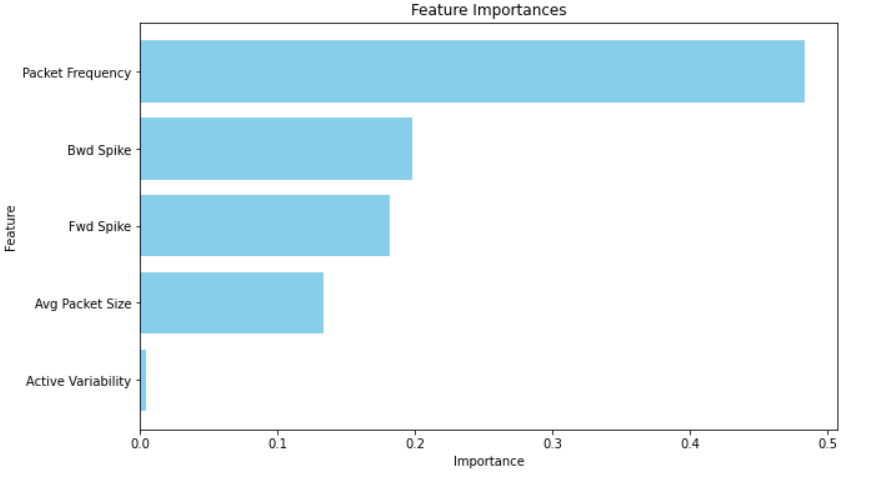
\includegraphics[height=4cm]{features_importance.png} 
    \caption{Feature Importance Analysis}
    \label{fig:features_importance}
\end{figure}


\subsection{Challenges encountered and how we solved them}
Throughout the implementation, several challenges we encountered several challenges:
\begin{itemize}
    \item \textbf{Path Issues:} Automating file handling during the \texttt{.pcap} to \texttt{.csv} conversion resolved errors related to incorrect file paths.
    \item \textbf{Data Imbalance:} Using SMOTE ensured balanced training data, reducing bias in the classification model.
    \item \textbf{Noise in Traffic Data:} Isolating YouTube streams and cleaning the dataset minimized unrelated traffic.
    \item \textbf{Hyperparameter Tuning:} Adjusting hyperparameters and improving feature engineering helped improve classification accuracy and reduce overfitting.
    \item \textbf{Data Quality Issues:} Removing blank data and refining derived features such as \texttt{Spike Difference} enhanced the consistency of the dataset.
\end{itemize}

